A continuación se presentan los resultados obtenidos para los experimentos de ordenamiento y multiplicación de matrices. Cada figura incluye una breve descripción de las observaciones más relevantes.

\subsection*{Algoritmos de ordenamiento}

La \Cref{fig:tiempo_sorting} muestra el tiempo de ejecución en función del tamaño de entrada $n$ para cada algoritmo de ordenamiento evaluado. En general, todos los algoritmos escalan de manera muy similar, siendo Merge Sort \cite{geeksforgeeks-mergesort} el que más se demora en todos los casos, seguido por Quick Sort \cite{geeksforgeeks-quicksort3way} con un tiempo inferior pero aún por encima de \texttt{std::sort}, que resultó ser el algoritmo más eficiente. Sin embargo, existen excepciones notables según el tipo de ordenamiento: cuando los datos están en orden ascendente, Merge Sort presenta un tiempo inicial muy elevado comparado con los otros algoritmos que comienzan con tiempos similares; en contraste, cuando los datos están en orden descendente, \texttt{std::sort} muestra un mejor desempeño inicial.

\begin{figure}[H]
    \centering
    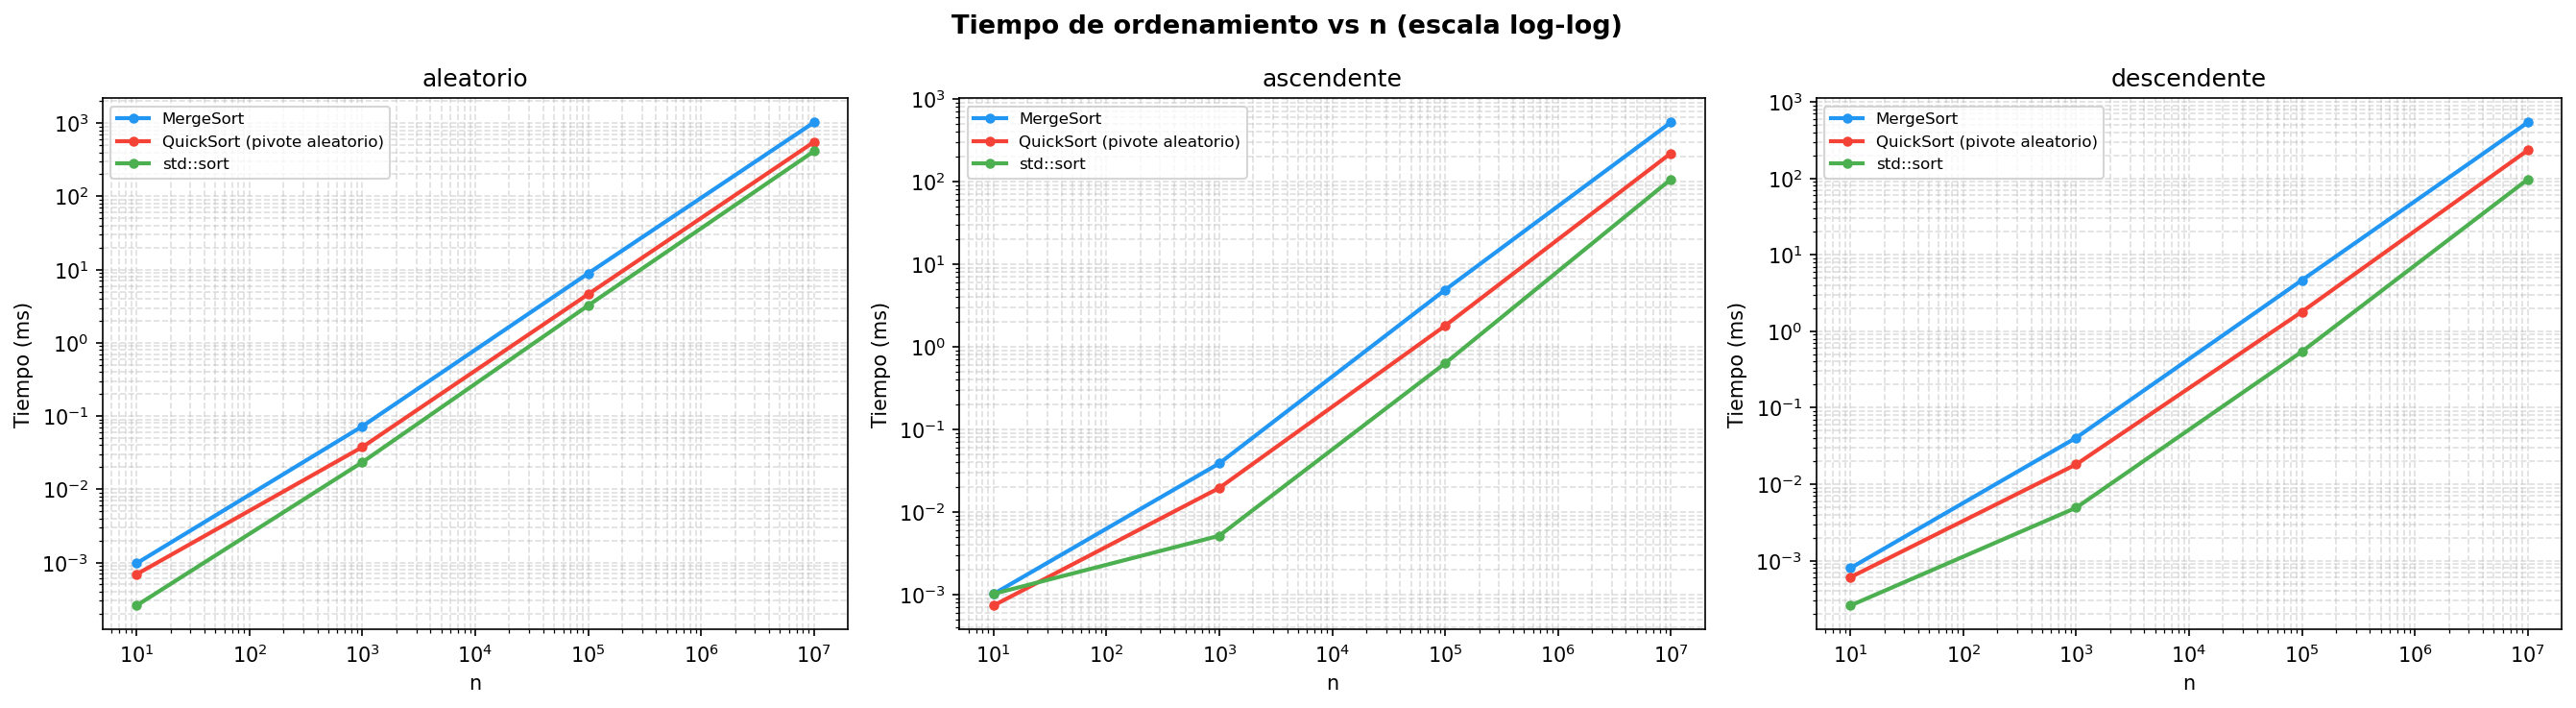
\includegraphics[width=\linewidth]{../code/sorting/data/plots/tiempo_vs_n_subplots_tipo.png}
    \caption{Tiempo de ejecución vs.\ tamaño de entrada $n$ para los algoritmos de ordenamiento evaluados.}
    \label{fig:tiempo_sorting}
\end{figure}

La \Cref{fig:memoria_sorting} presenta el uso de memoria en función del tamaño de entrada para cada tipo de algoritmo. Se aprecia que algoritmos recursivos como Merge Sort \cite{geeksforgeeks-mergesort} presentan un mayor consumo de memoria debido a la pila de llamadas y a la necesidad de arreglos auxiliares.

\begin{figure}[H]
    \centering
    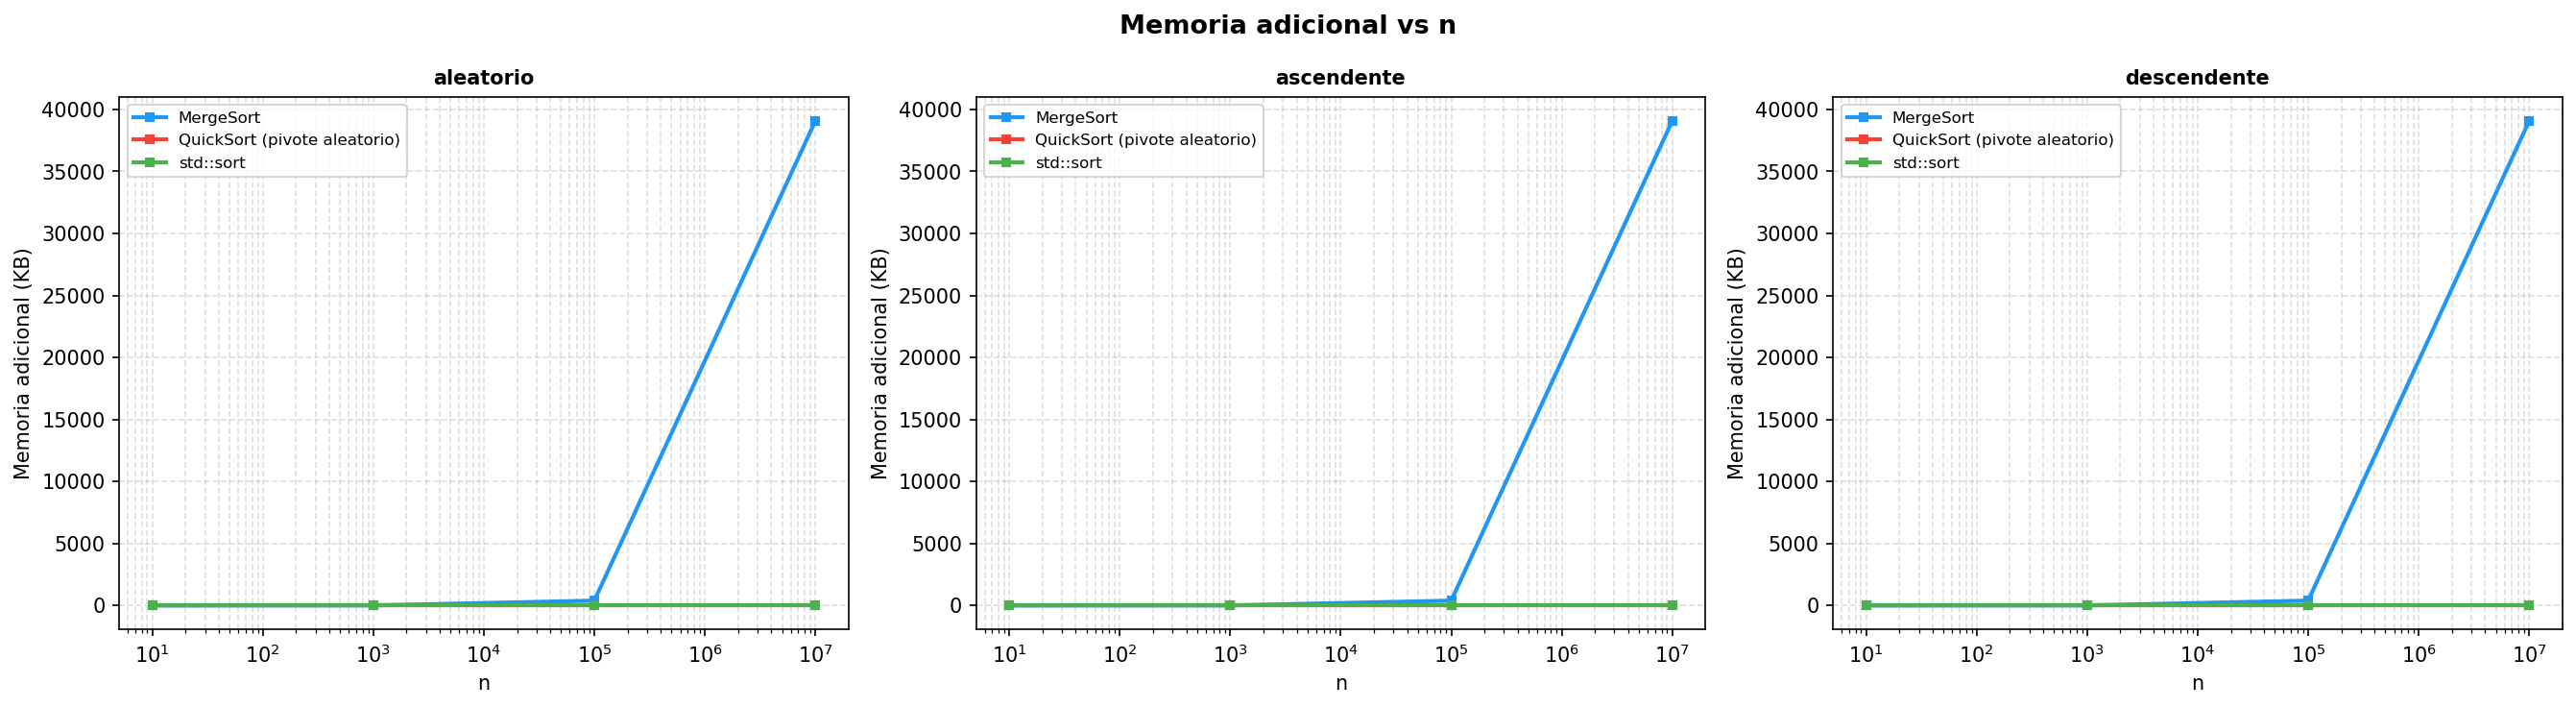
\includegraphics[width=\linewidth]{../code/sorting/data/plots/memoria_vs_n_subplots_tipo.png}
    \caption{Uso de memoria vs.\ tamaño de entrada $n$ para los algoritmos de ordenamiento, agrupados por tipo.}
    \label{fig:memoria_sorting}
\end{figure}

La \Cref{fig:heatmap_sorting} muestra un mapa de calor del tiempo de ejecución para $n = 100.000$ entre los distintos algoritmos. Esta visualización permite comparar de forma directa el rendimiento relativo de cada algoritmo en un tamaño de entrada fijo y de mayor escala.

\begin{figure}[H]
    \centering
    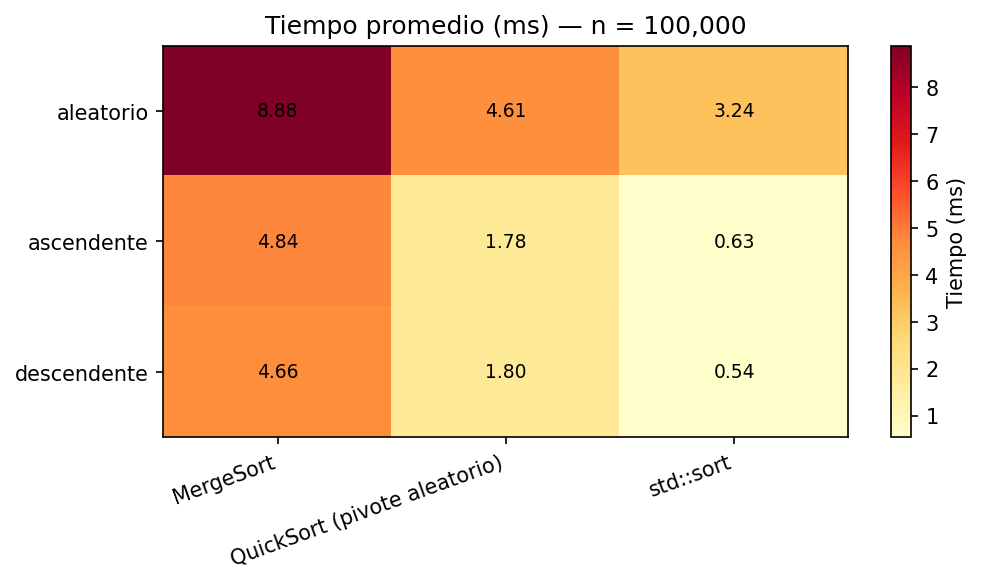
\includegraphics[width=0.85\linewidth]{../code/sorting/data/plots/heatmap_tiempo_n100000.png}
    \caption{Mapa de calor del tiempo de ejecución para $n = 100.000$ entre los algoritmos de ordenamiento.}
    \label{fig:heatmap_sorting}
\end{figure}

\subsection*{Multiplicación de matrices}

La \Cref{fig:tiempo_matmul} presenta el tiempo de ejecución en función del tamaño de la matriz $n \times n$ para cada algoritmo de multiplicación evaluado. Se observa que el algoritmo de Strassen \cite{geeksforgeeks-strassen} reduce el tiempo de ejecución para matrices de mayor tamaño respecto al algoritmo cúbico clásico, confirmando su ventaja asintótica \cite{algorithm2e}.

\begin{figure}[H]
    \centering
    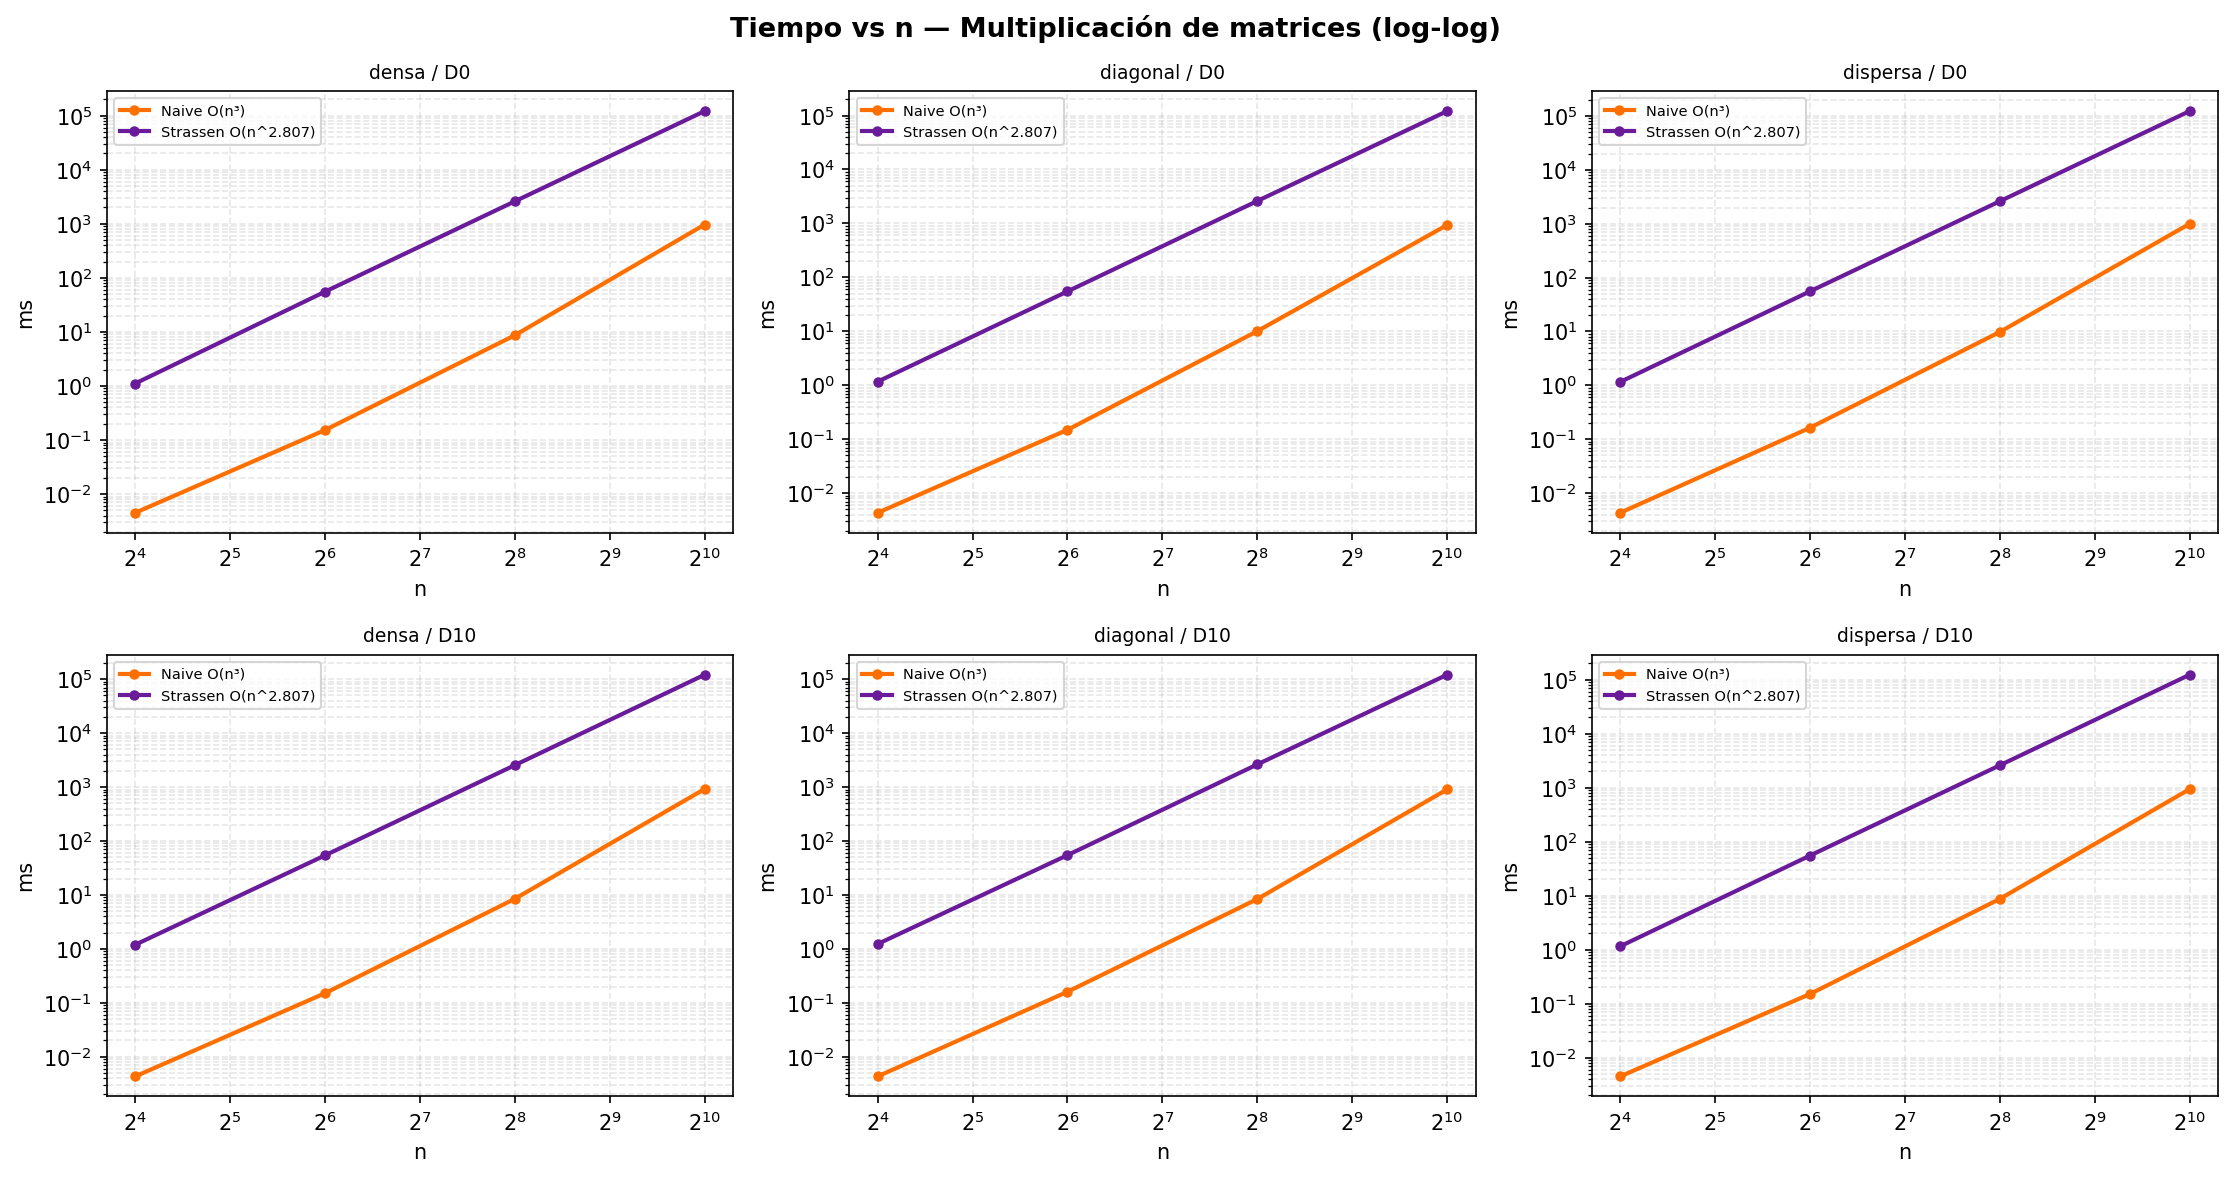
\includegraphics[width=\linewidth]{../code/matrix_multiplication/data/plots/tiempo_vs_n_subplots.png}
    \caption{Tiempo de ejecución vs.\ tamaño de matriz $n$ para los algoritmos de multiplicación de matrices, agrupados por tipo.}
    \label{fig:tiempo_matmul}
\end{figure}

La \Cref{fig:memoria_matmul} muestra el uso de memoria en función de $n$ para cada algoritmo de multiplicación. El algoritmo de Strassen \cite{geeksforgeeks-strassen} exhibe un mayor consumo de memoria producto de las submatrices intermedias generadas en cada nivel de recursión, como se preveia.

\begin{figure}[H]
    \centering
    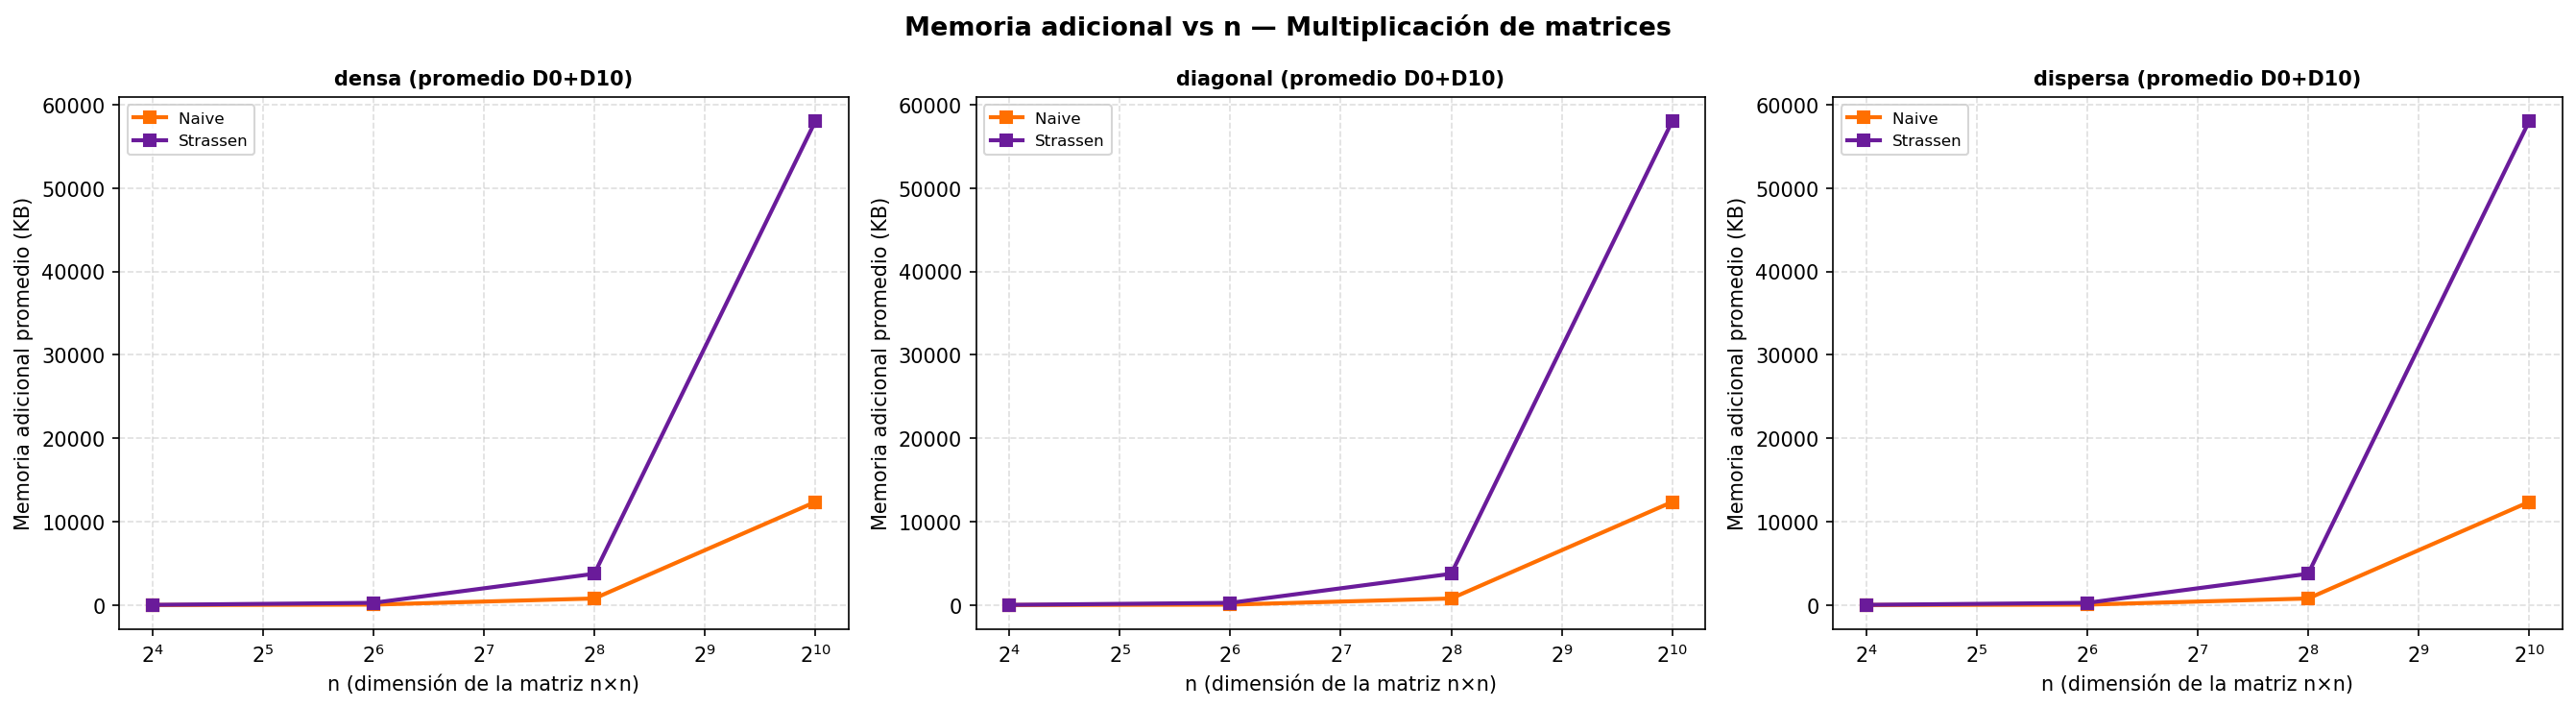
\includegraphics[width=\linewidth]{../code/matrix_multiplication/data/plots/memoria_vs_n_por_tipo.png}
    \caption{Uso de memoria vs.\ tamaño de matriz $n$ para los algoritmos de multiplicación de matrices, por tipo.}
    \label{fig:memoria_matmul}
\end{figure}